\documentclass[]{article}
\usepackage{lmodern}
\usepackage{amssymb,amsmath}
\usepackage{ifxetex,ifluatex}
\usepackage{fixltx2e} % provides \textsubscript
\ifnum 0\ifxetex 1\fi\ifluatex 1\fi=0 % if pdftex
  \usepackage[T1]{fontenc}
  \usepackage[utf8]{inputenc}
\else % if luatex or xelatex
  \ifxetex
    \usepackage{mathspec}
  \else
    \usepackage{fontspec}
  \fi
  \defaultfontfeatures{Ligatures=TeX,Scale=MatchLowercase}
\fi
% use upquote if available, for straight quotes in verbatim environments
\IfFileExists{upquote.sty}{\usepackage{upquote}}{}
% use microtype if available
\IfFileExists{microtype.sty}{%
\usepackage{microtype}
\UseMicrotypeSet[protrusion]{basicmath} % disable protrusion for tt fonts
}{}
\usepackage[margin=1in]{geometry}
\usepackage{hyperref}
\hypersetup{unicode=true,
            pdftitle={Estatística Básica},
            pdfauthor={Luan Fiorentin},
            pdfborder={0 0 0},
            breaklinks=true}
\urlstyle{same}  % don't use monospace font for urls
\usepackage{color}
\usepackage{fancyvrb}
\newcommand{\VerbBar}{|}
\newcommand{\VERB}{\Verb[commandchars=\\\{\}]}
\DefineVerbatimEnvironment{Highlighting}{Verbatim}{commandchars=\\\{\}}
% Add ',fontsize=\small' for more characters per line
\usepackage{framed}
\definecolor{shadecolor}{RGB}{248,248,248}
\newenvironment{Shaded}{\begin{snugshade}}{\end{snugshade}}
\newcommand{\KeywordTok}[1]{\textcolor[rgb]{0.13,0.29,0.53}{\textbf{#1}}}
\newcommand{\DataTypeTok}[1]{\textcolor[rgb]{0.13,0.29,0.53}{#1}}
\newcommand{\DecValTok}[1]{\textcolor[rgb]{0.00,0.00,0.81}{#1}}
\newcommand{\BaseNTok}[1]{\textcolor[rgb]{0.00,0.00,0.81}{#1}}
\newcommand{\FloatTok}[1]{\textcolor[rgb]{0.00,0.00,0.81}{#1}}
\newcommand{\ConstantTok}[1]{\textcolor[rgb]{0.00,0.00,0.00}{#1}}
\newcommand{\CharTok}[1]{\textcolor[rgb]{0.31,0.60,0.02}{#1}}
\newcommand{\SpecialCharTok}[1]{\textcolor[rgb]{0.00,0.00,0.00}{#1}}
\newcommand{\StringTok}[1]{\textcolor[rgb]{0.31,0.60,0.02}{#1}}
\newcommand{\VerbatimStringTok}[1]{\textcolor[rgb]{0.31,0.60,0.02}{#1}}
\newcommand{\SpecialStringTok}[1]{\textcolor[rgb]{0.31,0.60,0.02}{#1}}
\newcommand{\ImportTok}[1]{#1}
\newcommand{\CommentTok}[1]{\textcolor[rgb]{0.56,0.35,0.01}{\textit{#1}}}
\newcommand{\DocumentationTok}[1]{\textcolor[rgb]{0.56,0.35,0.01}{\textbf{\textit{#1}}}}
\newcommand{\AnnotationTok}[1]{\textcolor[rgb]{0.56,0.35,0.01}{\textbf{\textit{#1}}}}
\newcommand{\CommentVarTok}[1]{\textcolor[rgb]{0.56,0.35,0.01}{\textbf{\textit{#1}}}}
\newcommand{\OtherTok}[1]{\textcolor[rgb]{0.56,0.35,0.01}{#1}}
\newcommand{\FunctionTok}[1]{\textcolor[rgb]{0.00,0.00,0.00}{#1}}
\newcommand{\VariableTok}[1]{\textcolor[rgb]{0.00,0.00,0.00}{#1}}
\newcommand{\ControlFlowTok}[1]{\textcolor[rgb]{0.13,0.29,0.53}{\textbf{#1}}}
\newcommand{\OperatorTok}[1]{\textcolor[rgb]{0.81,0.36,0.00}{\textbf{#1}}}
\newcommand{\BuiltInTok}[1]{#1}
\newcommand{\ExtensionTok}[1]{#1}
\newcommand{\PreprocessorTok}[1]{\textcolor[rgb]{0.56,0.35,0.01}{\textit{#1}}}
\newcommand{\AttributeTok}[1]{\textcolor[rgb]{0.77,0.63,0.00}{#1}}
\newcommand{\RegionMarkerTok}[1]{#1}
\newcommand{\InformationTok}[1]{\textcolor[rgb]{0.56,0.35,0.01}{\textbf{\textit{#1}}}}
\newcommand{\WarningTok}[1]{\textcolor[rgb]{0.56,0.35,0.01}{\textbf{\textit{#1}}}}
\newcommand{\AlertTok}[1]{\textcolor[rgb]{0.94,0.16,0.16}{#1}}
\newcommand{\ErrorTok}[1]{\textcolor[rgb]{0.64,0.00,0.00}{\textbf{#1}}}
\newcommand{\NormalTok}[1]{#1}
\usepackage{graphicx,grffile}
\makeatletter
\def\maxwidth{\ifdim\Gin@nat@width>\linewidth\linewidth\else\Gin@nat@width\fi}
\def\maxheight{\ifdim\Gin@nat@height>\textheight\textheight\else\Gin@nat@height\fi}
\makeatother
% Scale images if necessary, so that they will not overflow the page
% margins by default, and it is still possible to overwrite the defaults
% using explicit options in \includegraphics[width, height, ...]{}
\setkeys{Gin}{width=\maxwidth,height=\maxheight,keepaspectratio}
\IfFileExists{parskip.sty}{%
\usepackage{parskip}
}{% else
\setlength{\parindent}{0pt}
\setlength{\parskip}{6pt plus 2pt minus 1pt}
}
\setlength{\emergencystretch}{3em}  % prevent overfull lines
\providecommand{\tightlist}{%
  \setlength{\itemsep}{0pt}\setlength{\parskip}{0pt}}
\setcounter{secnumdepth}{0}
% Redefines (sub)paragraphs to behave more like sections
\ifx\paragraph\undefined\else
\let\oldparagraph\paragraph
\renewcommand{\paragraph}[1]{\oldparagraph{#1}\mbox{}}
\fi
\ifx\subparagraph\undefined\else
\let\oldsubparagraph\subparagraph
\renewcommand{\subparagraph}[1]{\oldsubparagraph{#1}\mbox{}}
\fi

%%% Use protect on footnotes to avoid problems with footnotes in titles
\let\rmarkdownfootnote\footnote%
\def\footnote{\protect\rmarkdownfootnote}

%%% Change title format to be more compact
\usepackage{titling}

% Create subtitle command for use in maketitle
\newcommand{\subtitle}[1]{
  \posttitle{
    \begin{center}\large#1\end{center}
    }
}

\setlength{\droptitle}{-2em}

  \title{Estatística Básica}
    \pretitle{\vspace{\droptitle}\centering\huge}
  \posttitle{\par}
  \subtitle{Lista 1 GABARITO - Introdução à Estatística e Amostragem}
  \author{Luan Fiorentin}
    \preauthor{\centering\large\emph}
  \postauthor{\par}
      \predate{\centering\large\emph}
  \postdate{\par}
    \date{2019-03-05}

\usepackage{amsmath} \usepackage{float} \usepackage{bm}

\begin{document}
\maketitle

\begin{enumerate}
\def\labelenumi{\arabic{enumi}.}
\tightlist
\item
  Defina o que é população e o que é amostra. Qual a diferença entre
  parâmetro populacional e estatística amostral?
\end{enumerate}

\begin{Shaded}
\begin{Highlighting}[]
\CommentTok{# População é uma coleção de indivíduos, itens ou objetos}
\CommentTok{# que possuem uma característica de interesse.}
\CommentTok{# Amostra é subconjunto da população, mas que possui uma característica}
\CommentTok{# de interesse também. Em geral, a amostra possui dimensões bem menores que o tamanho }
\CommentTok{# da população.}
\CommentTok{# Parâmetro populacional é uma característica numérica que descreve a população.}
\CommentTok{# Estatística é uma característica numérica calculada com base na amostra.}
\end{Highlighting}
\end{Shaded}

\begin{enumerate}
\def\labelenumi{\arabic{enumi}.}
\setcounter{enumi}{1}
\tightlist
\item
  Nos itens abaixo indique se na situação temos uma estatística (E) ou
  um parâmetro (P).

  \begin{enumerate}
  \def\labelenumii{(\alph{enumii})}
  \tightlist
  \item
    Tem-se interesse na altura média dos jogadores de basquete
    profissional no Brasil. São medidas as alturas de 30\% dos jogadores
    profissionais dos diversos times nacionais, e então a média é
    calculada.
  \item
    Tem-se interesse na altura média dos jogadores de basquete
    profissional no Brasil. São medidas as alturas de todos os jogadores
    profissionais dos diversos times nacionais, e então a média é
    calculada.
  \item
    O objetivo é obter a biomassa (peso total) de determinada espécie de
    planta em uma floresta. São pesadas todas as folhas caídas desta
    espécie, coletados em conglomerados amostrais com 1 m² cada um
    distribuídos aleatoriamente de forma a cobrir 1\% da área da
    floresta.
  \item
    Tem-se interesse no comprimento médio dos peixes criados em um
    tanque de cultivo. Na despesca o tanque é esgotado, os peixes são
    abatidos e medidos, e finalmente se calcula uma média.
  \item
    Foi perguntado para 100 estudantes, selecionados aleatoriamente, o
    tempo médio de espera na fila do RU. O resultado foi de 20 minutos.
  \item
    Em um estudo de todos os 2223 passageiros do Titanic, verificou-se
    que 706 sobreviveram quando ele afundou.
  \item
    Há interesse em se estudar a altura de uma espécie de árvore e, após
    medir 10 delas entre várias presentes no local da coleta, calculamos
    que, em média, uma árvore mede 4,14 metros.
  \item
    O Senado atual de um país é composto por 87 homens e 13 mulheres.
  \end{enumerate}
\end{enumerate}

\begin{Shaded}
\begin{Highlighting}[]
\NormalTok{(resp2)}
\end{Highlighting}
\end{Shaded}

\begin{verbatim}
##   Alternativa Resposta
## 1           a        E
## 2           b        P
## 3           c        E
## 4           d        P
## 5           e        E
## 6           f        P
## 7           g        E
## 8           h        P
\end{verbatim}

\begin{enumerate}
\def\labelenumi{\arabic{enumi}.}
\setcounter{enumi}{2}
\tightlist
\item
  Indique que tipo de amostragem (aleatória simples, sistemática,
  estratificada ou conglomerado) está sendo utilizada em cada um dos
  casos descritos abaixo.

  \begin{enumerate}
  \def\labelenumii{(\alph{enumii})}
  \tightlist
  \item
    Um bairro com 1000 quadras é dividido em 1000 parcelas com 1 quadra
    cada. São sorteadas 40 parcelas e todos os moradores (maiores de
    idade) são questionados sobre a eficácia das obras da prefeitura
    naquele bairro.
  \item
    Em uma área arborizada são escolhidas dez árvores ao acaso, e os
    diâmetros delas são então medidos.
  \item
    Em uma indústria de mineração, sedimentos são transportados sobre
    uma esteira a uma determinada velocidade. Um pesquisador parado ao
    lado da esteira interrompe seu andamento e coleta uma amostra de 5
    em 5 minutos.
  \item
    Interessado em estudar os pesos de uma espécie de ave, um
    pesquisador seleciona ao acaso 30 fêmeas e também 30 machos.
  \item
    Uma Universidade fez um estudo sobre o hábito de bebida dos
    estudantes, selecionando aleatoriamente 10 classes diferentes, e
    entrevistando todos os alunos de cada uma das classes.
  \item
    Um Economista está estudando o efeito da educação sobre o salário, e
    realiza uma pesquisa com 150 trabalhadores selecionados
    aleatoriamente de cada uma das seguintes categorias: menos do que o
    ensino médio, ensino médio, mais do que o ensino médio.
  \end{enumerate}
\end{enumerate}

\begin{Shaded}
\begin{Highlighting}[]
\NormalTok{resp3}
\end{Highlighting}
\end{Shaded}

\begin{verbatim}
##   Alternativa          Resposta
## 1           a      Conglomerado
## 2           b Aleatória Simples
## 3           c       Sistemática
## 4           d     Estratificada
## 5           e      Conglomerado
## 6           f     Estratificada
\end{verbatim}

\begin{enumerate}
\def\labelenumi{\arabic{enumi}.}
\setcounter{enumi}{3}
\tightlist
\item
  Classifique as variáveis em nominal (N), ordinal (O), discreta (D) ou
  contínua (C):

  \begin{enumerate}
  \def\labelenumii{(\alph{enumii})}
  \tightlist
  \item
    Medidas de diâmetro (mm) de um rolamento industrial.
  \item
    Número de ações da Petrobrás disponíveis no mercado financeiro em
    2013.
  \item
    Nomes de empresas de Curitiba com mais de 100 funcionários.
  \item
    Número de estudantes que frequentam o RU diariamente
  \item
    Temperatura das câmaras frias de uma indústria de pescado.
  \item
    Peso de algas coletadas em um determinado banco submerso.
  \item
    Avaliação em graus de qualidade (``bom'', ``razoável'', ``ruim'') de
    um equipamento industrial.
  \item
    Tempo que você dispenderá estudando para a prova de estatística.
  \item
    Grau de satisfação da população brasileira com relação ao trabalho
    de seu presidente (valores de 0 a 5, com 0 indicando totalmente
    insatisfeito e 5 totalmenet satisfeito).
  \end{enumerate}
\end{enumerate}

\begin{Shaded}
\begin{Highlighting}[]
\NormalTok{resp4}
\end{Highlighting}
\end{Shaded}

\begin{verbatim}
##   Alternativa Resposta
## 1           a        C
## 2           b        D
## 3           c        N
## 4           d        D
## 5           e        C
## 6           f        C
## 7           g        O
## 8           h        C
## 9           i        O
\end{verbatim}

\begin{enumerate}
\def\labelenumi{\arabic{enumi}.}
\setcounter{enumi}{4}
\tightlist
\item
  Um professor pergunta a cada um de seus alunos que ramo do
  conhecimento prefere estudar: Línguas e Literatura (LL), Ciências
  Exatas (CE), Ciências Físicas e Naturais (FN), Artes e Música (AM).
  Organize a distribuição das frequências com as respostas abaixo e
  construa um gráfico de barras.
\end{enumerate}

\begin{table}[H]
\centering
\begin{tabular}{ccccc}
\hline
AM & LL & FN & AM & FN \\
LL & LL & LL & LL & AM \\
FN & AM & CE & FN &    \\
CE & FN & FN & AM &    \\
CE & FN & CE & LL &    \\ \hline
\end{tabular}
\end{table}

\begin{Shaded}
\begin{Highlighting}[]
\CommentTok{# Frequência absoluta}
\NormalTok{(fa <-}\StringTok{ }\KeywordTok{addmargins}\NormalTok{(}\KeywordTok{table}\NormalTok{(da5)))}
\end{Highlighting}
\end{Shaded}

\begin{verbatim}
## da5
##  AM  CE  FN  LL Sum 
##   5   4   7   6  22
\end{verbatim}

\begin{Shaded}
\begin{Highlighting}[]
\CommentTok{# Frequência absoluta acumulada}
\NormalTok{(FA <-}\StringTok{ }\KeywordTok{cumsum}\NormalTok{(}\KeywordTok{round}\NormalTok{(}\KeywordTok{table}\NormalTok{(da5), }\DecValTok{2}\NormalTok{)))}
\end{Highlighting}
\end{Shaded}

\begin{verbatim}
## AM CE FN LL 
##  5  9 16 22
\end{verbatim}

\begin{Shaded}
\begin{Highlighting}[]
\CommentTok{# Gráfico de barras para frequência absoluta}
\CommentTok{# e absoluta acumulada}
\KeywordTok{par}\NormalTok{(}\DataTypeTok{mfrow =} \KeywordTok{c}\NormalTok{(}\DecValTok{1}\NormalTok{,}\DecValTok{2}\NormalTok{))}
\KeywordTok{barplot}\NormalTok{(}\KeywordTok{table}\NormalTok{(da5), }
        \DataTypeTok{ylim =} \KeywordTok{c}\NormalTok{(}\DecValTok{0}\NormalTok{,}\DecValTok{10}\NormalTok{), }
        \DataTypeTok{ylab =} \StringTok{"Frequência absoluta"}\NormalTok{, }
        \DataTypeTok{xlab =} \StringTok{"Área do conhecimento"}\NormalTok{)}
\KeywordTok{barplot}\NormalTok{(FA, }\DataTypeTok{ylim =} \KeywordTok{c}\NormalTok{(}\DecValTok{0}\NormalTok{,}\DecValTok{25}\NormalTok{), }
        \DataTypeTok{ylab =} \StringTok{"Frequência absoluta acumulada"}\NormalTok{, }
        \DataTypeTok{xlab =} \StringTok{"Área do conhecimento"}\NormalTok{)}
\end{Highlighting}
\end{Shaded}

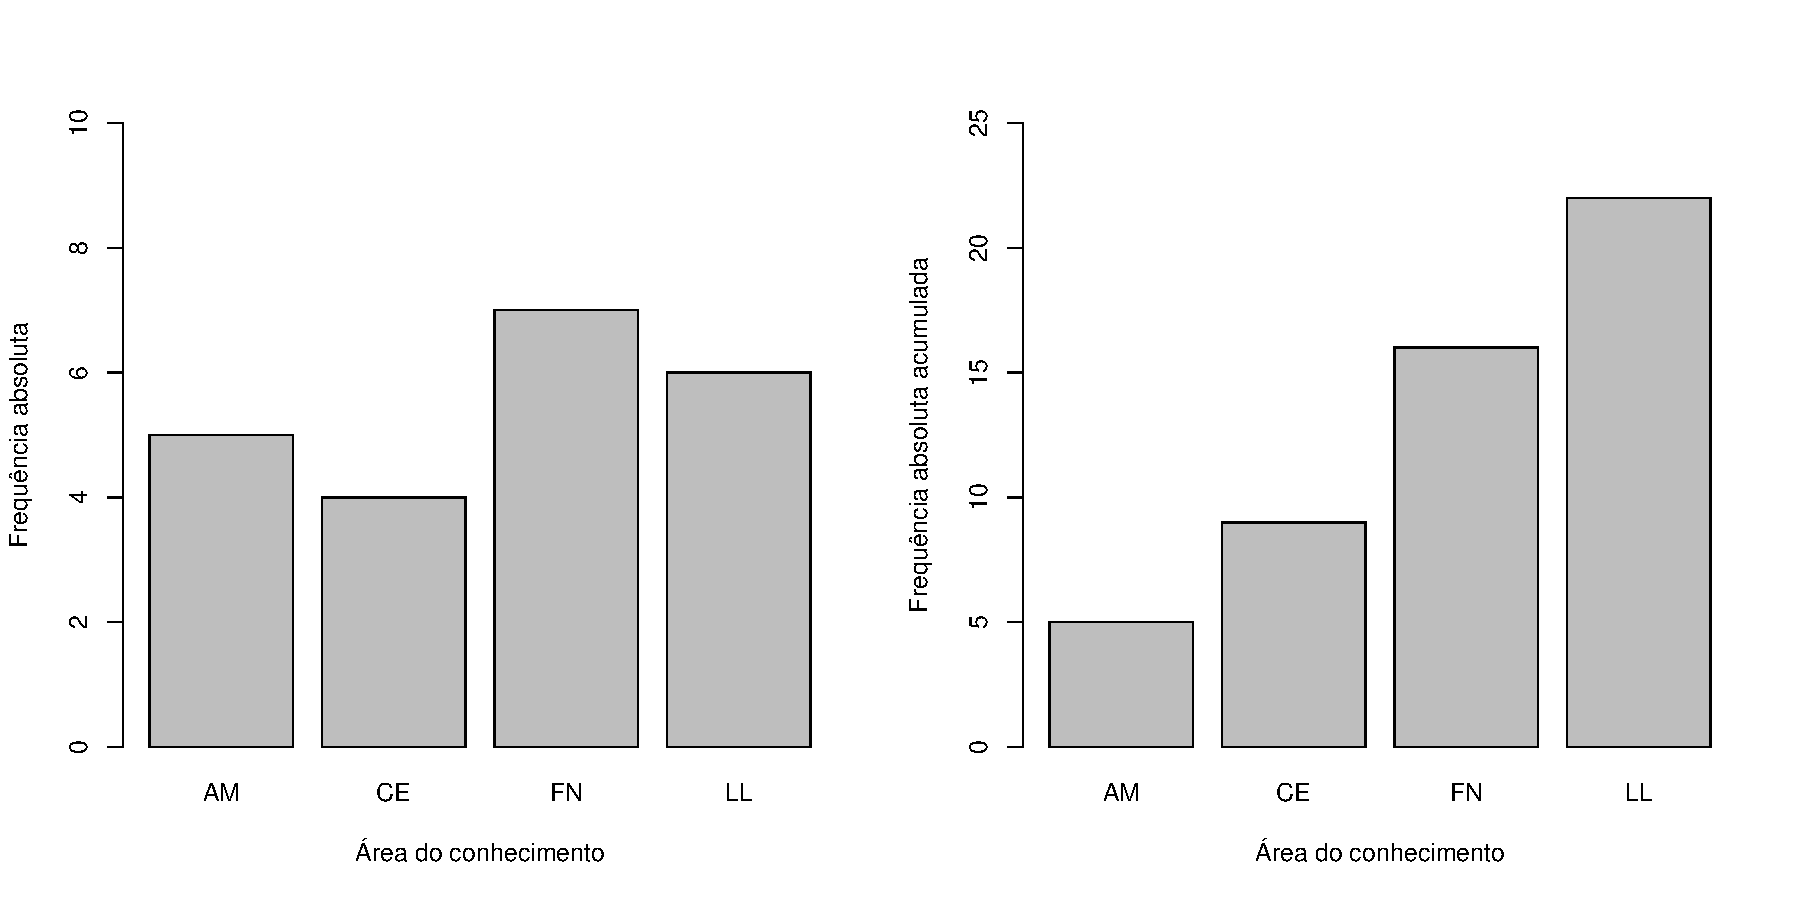
\includegraphics{Lista_1_Gabarito_files/figure-latex/unnamed-chunk-9-1.pdf}

\begin{enumerate}
\def\labelenumi{\arabic{enumi}.}
\setcounter{enumi}{5}
\tightlist
\item
  A tabela de distribuições de frequência abaixo apresenta o tempo (em
  minutos) que uma pessoa leva para encontrar um livro na estante de uma
  biblioteca, após consultar o sistema e saber o número de referência do
  livro.

  \begin{enumerate}
  \def\labelenumii{(\alph{enumii})}
  \tightlist
  \item
    Complete a tabela com as frequências: acumulada, relativa e relativa
    acumulada
  \item
    Em quantos minutos (intervalo de minutos) é mais comum as pessoas
    encontrarem o livro?
  \item
    Qual a porcentagem de pessoas que levam menos de 3 minutos para
    encontrar o livro?
  \item
    Quantas pessoas levam menos de 2 minutos para encontrar o livro?
  \item
    Qual o percentual de pessoas que levam entre 4 minutos (inclusive) e
    4,5 minutos?
  \item
    Qual o percentual de pessoas que levam no máximo 1 minuto para
    encontrar o livro?
  \end{enumerate}
\end{enumerate}

\begin{table}[H]
\centering
\begin{tabular}{cc}
\hline
Classes     & Frequência \\ \cline{1-2}
{[}0,5-1,0) & 1          \\
{[}1,0-1,5) & 3          \\
{[}1,5-2,0) & 22         \\
{[}2,0-2,5) & 115        \\
{[}2,5-3,0  & 263        \\
{[}3,0-3,5) & 287        \\
{[}3,5-4,0) & 99         \\
{[}4,0-4,5) & 32         \\ \hline
\end{tabular}
\end{table}

\begin{Shaded}
\begin{Highlighting}[]
\CommentTok{# (a)}
\NormalTok{da6}
\end{Highlighting}
\end{Shaded}

\begin{verbatim}
##     Classes Freq Fac    fr  Frac
## 1 [0,5-1,0)    1   1 0.001 0.001
## 2 [1,0-1,5)    3   4 0.004 0.005
## 3 [1,5-2,0)   22  26 0.027 0.032
## 4 [2,0-2,5)  115 141 0.140 0.172
## 5 [2,5-3,0)  263 404 0.320 0.492
## 6 [3,0-3,5)  287 691 0.349 0.841
## 7 [3,5-4,0)   99 790 0.120 0.961
## 8 [4,0-4,5)   32 822 0.039 1.000
\end{verbatim}

\begin{Shaded}
\begin{Highlighting}[]
\CommentTok{# (b)}
\CommentTok{# Entre 3,0 e 3,5 minutos.}

\CommentTok{# (c)}
\CommentTok{# 49,2 %}

\CommentTok{# (d)}
\CommentTok{# 26 pessoas}

\CommentTok{# (e)}
\CommentTok{# 3,9%}

\CommentTok{# (f)}
\CommentTok{# 0,1%}
\end{Highlighting}
\end{Shaded}

\begin{enumerate}
\def\labelenumi{\arabic{enumi}.}
\setcounter{enumi}{6}
\tightlist
\item
  Construa uma tabela com as distribuições de frequência absoluta,
  relativa, absoluta acumulada e relativa acumulada usando a amostra do
  número de páginas de livros infanto-juvenis dada ma sequência.
\end{enumerate}

\begin{table}[H]
\centering
\begin{tabular}{cccccccccc}
\cline{1-10}
46 & 46 & 53 & 30 & 62 & 50 & 69 & 49 & 58 & 65 \\
62 & 52 & 44 & 38 & 33 & 60 & 50 & 39 & 53 & 50 \\
64 & 53 & 45 & 38 & 31 & 41 & 56 & 54 & 38 & 42 \\
31 & 38 & 66 & 29 & 41 & 55 & 43 & 50 & 40 & 45 \\ \cline{1-10}
\end{tabular}
\end{table}

Construa um histograma com a densidade de frequência. O que você pode
interpretar destes dados a partir da tabela e dos gráficos?

\begin{Shaded}
\begin{Highlighting}[]
\NormalTok{da71}
\end{Highlighting}
\end{Shaded}

\begin{verbatim}
##         Freq. Freq. ac. Freq. rel. Freq. rel. ac. Dens.
## [24,30)     1         1      0.025          0.025 0.004
## [30,36)     4         5      0.100          0.125 0.017
## [36,42)     8        13      0.200          0.325 0.033
## [42,48)     7        20      0.175          0.500 0.029
## [48,54)     9        29      0.225          0.725 0.038
## [54,60)     4        33      0.100          0.825 0.017
## [60,66)     5        38      0.125          0.950 0.021
## [66,72]     2        40      0.050          1.000 0.008
\end{verbatim}

\begin{Shaded}
\begin{Highlighting}[]
\KeywordTok{par}\NormalTok{(}\DataTypeTok{mfrow =} \KeywordTok{c}\NormalTok{(}\DecValTok{1}\NormalTok{,}\DecValTok{2}\NormalTok{))}
\KeywordTok{hist}\NormalTok{(da7, }\DataTypeTok{breaks =} \KeywordTok{seq}\NormalTok{(}\DecValTok{24}\NormalTok{,}\DecValTok{72}\NormalTok{,}\DecValTok{6}\NormalTok{), }
     \DataTypeTok{ylim =} \KeywordTok{c}\NormalTok{(}\DecValTok{0}\NormalTok{,}\DecValTok{12}\NormalTok{), }\DataTypeTok{xlim =} \KeywordTok{c}\NormalTok{(}\DecValTok{20}\NormalTok{,}\DecValTok{80}\NormalTok{), }
     \DataTypeTok{xlab =} \StringTok{"Número de páginas"}\NormalTok{, }
     \DataTypeTok{ylab =} \StringTok{"Frequência absoluta"}\NormalTok{, }
     \DataTypeTok{main =} \StringTok{""}\NormalTok{)}
\KeywordTok{hist}\NormalTok{(da7, }\DataTypeTok{breaks =} \KeywordTok{seq}\NormalTok{(}\DecValTok{24}\NormalTok{,}\DecValTok{72}\NormalTok{,}\DecValTok{6}\NormalTok{), }\DataTypeTok{probability =}\NormalTok{ T, }
     \DataTypeTok{ylim =} \KeywordTok{c}\NormalTok{(}\DecValTok{0}\NormalTok{,}\FloatTok{0.05}\NormalTok{), }\DataTypeTok{xlim =} \KeywordTok{c}\NormalTok{(}\DecValTok{20}\NormalTok{,}\DecValTok{80}\NormalTok{), }
     \DataTypeTok{xlab =} \StringTok{"Número de páginas"}\NormalTok{, }
     \DataTypeTok{ylab =} \StringTok{"Densidade de frequência", }
\StringTok{     main = "")}
\end{Highlighting}
\end{Shaded}

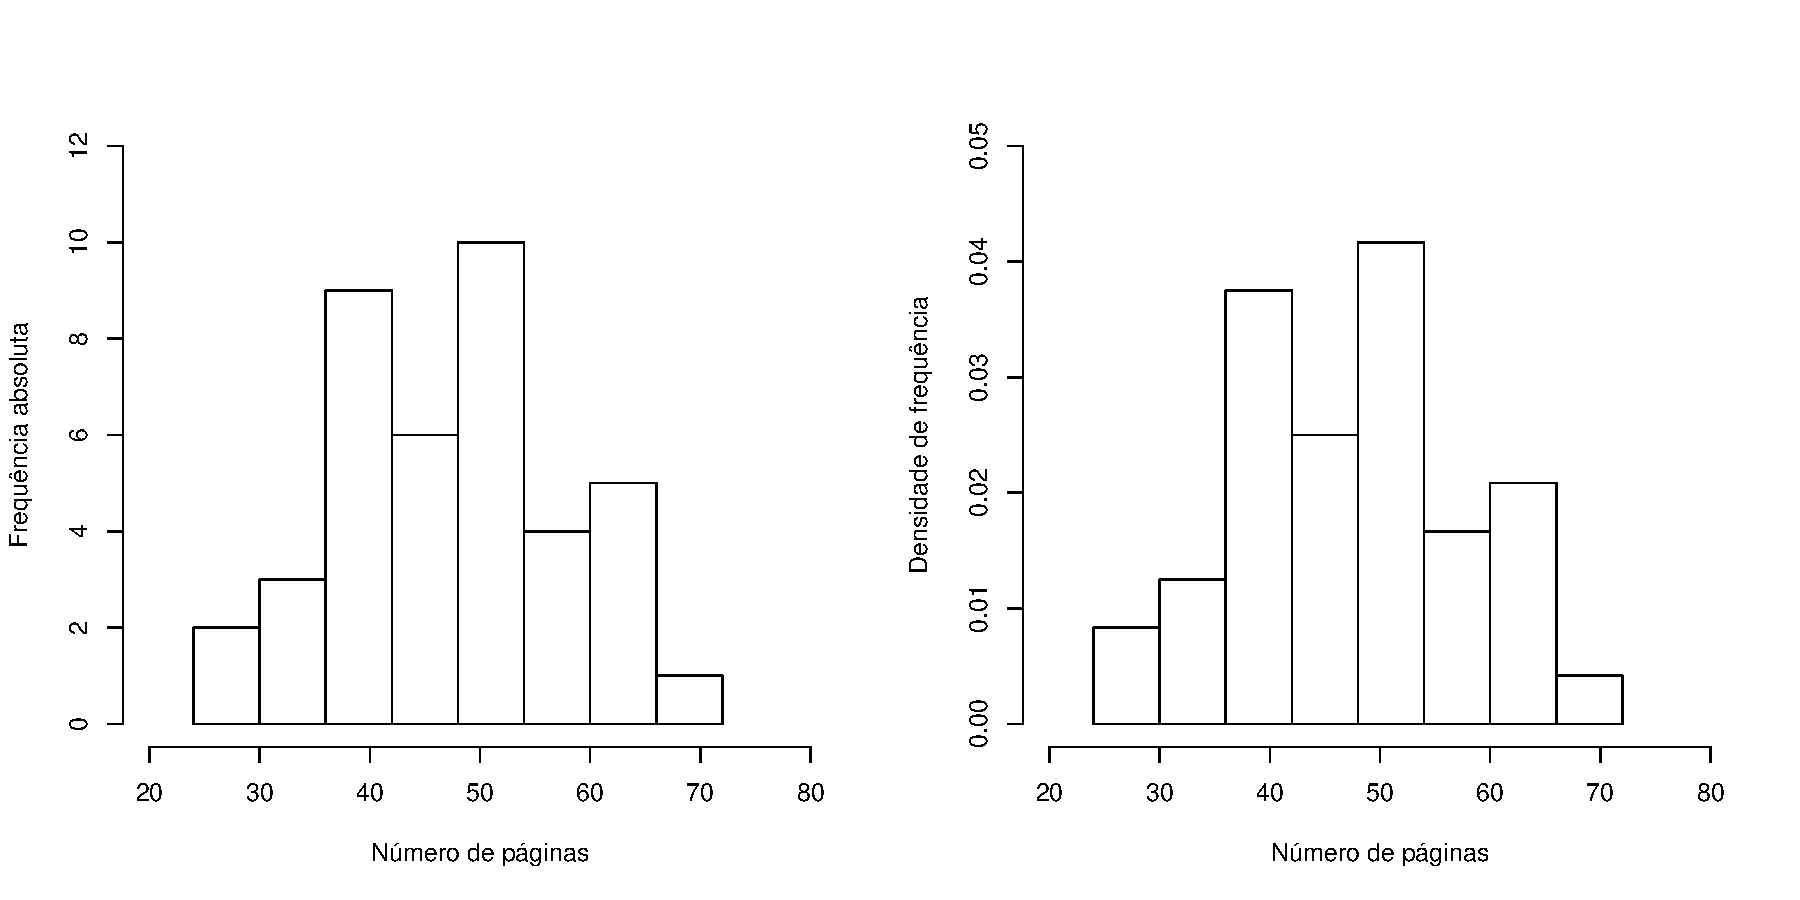
\includegraphics{Lista_1_Gabarito_files/figure-latex/unnamed-chunk-13-1.pdf}

\begin{enumerate}
\def\labelenumi{\arabic{enumi}.}
\setcounter{enumi}{7}
\tightlist
\item
  Qual a diferença entre um gráfico de barras e um histograma?
\end{enumerate}

\begin{Shaded}
\begin{Highlighting}[]
\CommentTok{# O gráfico de barras é uma representação gráfica de uma tabela de frequência}
\CommentTok{# para dados qualitativos.}
\CommentTok{# O histograma é uma representação gráfica de uma tabela de frequência para}
\CommentTok{# dados quantitativos, com intervalos de classes determinados.}
\CommentTok{# O histograma deve ter as barras unidas para representar uma área. }
\end{Highlighting}
\end{Shaded}


\end{document}
